\documentclass[14pt, a4paper]{article}

\usepackage[T2A]{fontenc}
\usepackage[utf8]{inputenc}
\usepackage[english,russian]{babel}

\usepackage{graphicx}
\usepackage{float}
\graphicspath{{./images/}}

\begin{document}
    \thispagestyle{empty}

    \begin{center}
        Министерство науки и высшего образования Российской Федерации

        Федеральное государственно автономное образовательное учреждение высшего образования

        <<Омский государственный технический университет>>

        \vspace{1cm}
        Факультет информационных технологий и компьютерных систем

        Кафедра <<Прикладная математика и фундаметральная информатика>>

        \vspace{3cm}
        \textbf{Расчётно-графическая работа}

        по дисциплине <<Практикум по программированию>>
    \end{center}
    
    \vspace{3cm}
    \begin{flushright}    
        \begin{tabular}{ r r }
            Студента & Курпенова Куата Ибраимовича \\
            \cline{2-2}
            & \tiny{фамилия, имя, отчество полностью} \\

            Курс & 2, группа ФИТ-212 \\
            \cline{2-2}
            Направление & 02.03.02 Прикладная математика \\
            \cline{2-2}
            & и фундаментальная информатика \\
            \cline{2-2}
            & \tiny{код, наименование} \\
            
            Руководитель & ст. преподаватель \\
            \cline{2-2}
            & \tiny{должность, ученая степень, звание} \\
            & Шарун И. В. \\
            \cline{2-2}
            & \tiny{фамилия, инициалы} \\
            
            Выполнил & \\
            \cline{2-2}
            & \tiny{дата, подпись студента} \\
        \end{tabular}

        \vspace{1cm}

        \begin{tabular}{ | c | c | }
            \hline
            Итоговый рейтинг & \\
            \hline
        \end{tabular}
    \end{flushright}
    
    \vspace*{\fill}
    \begin{center}
        Омск 2022
    \end{center}

    \newpage

    \tableofcontents

    \newpage

    \section{Введение}

    Анализ данных - область математики и информатики, занимающаяся построением и исследованием наиболее общих математических методов и вычислительных алгоритмов извлечения знаний из экспериментальных (в широком смысле) данных. Анализ данных — это не просто обработка информации после ее получения и сбора, это средство проверки гипотез. Цель любого анализа данных — понимание исследуемой ситуации целиком (выявление тенденций, в том числе негативных отклонений от плана, прогнозирование и получение рекомендации). Для достижения этой цели ставятся следующие задачи анализа данных:

    \begin{itemize}
        \item сбор информации
        \item структуризация информации
        \item выявление закономерностей, анализ
        \item прогнозирование и получение рекомендаций
    \end{itemize}

    Сейчас аналитика применяется практически во всех сферах: маркетинг, медицина, таргетированная реклама, банковская сфера и т.д. Грамотный аналитик данных в любой компании становится ключевой фигурой. Специалист по анализу данных это тот работник, который программирует лучше любого специалиста по статистике, и знает статистику лучше любого программиста, в бизнес-процессах разбирается лучше руководителя.

    Самый популярный инструмент дата сайентиста это, бесспорно, язык программирования python. В данной работе он был использован, так как и  ключевая для анализа данных библиотека pandas. Pandas содержит огромное количество методов работы с данными: от импорта датасета до построения графиков, вывода всевозможных характеристик.

    \subsection{Поиск и загрузка данных}
    В данной работе я использовал датасет <<Dairy queen menu nutrition>>. Этот датасет описывает питание - продукты, калории, доли полезных веществ в них.

    \subsection{Разведывательный анализ данных}
    
    \begin{figure}[H]
        \centering
        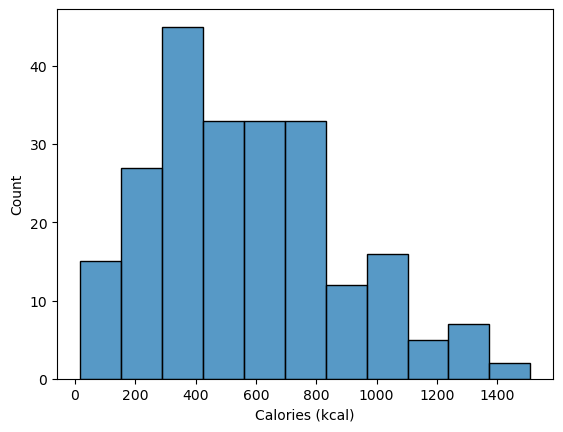
\includegraphics[width=0.75\textwidth]{images/histogram.png}
        \caption{Гистограмма распределения по столбцу <<Calories (kcal)>>}
    \end{figure}

    \begin{figure}[H]
        \centering
        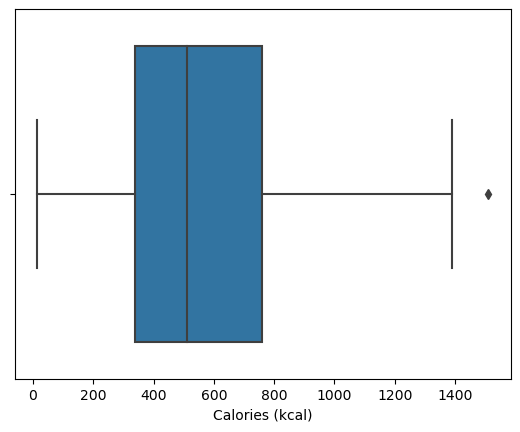
\includegraphics[width=0.75\textwidth]{images/boxplot.png}
        \caption{Диаграмма размаха по столбцу <<Calories (kcal)>>}
    \end{figure}

    \begin{figure}[H]
        \centering
        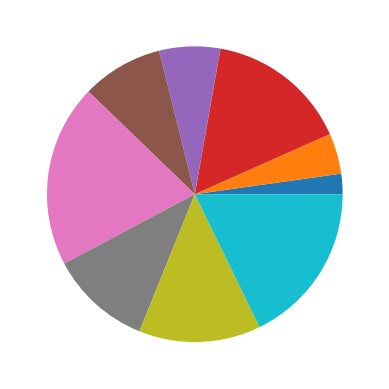
\includegraphics[width=0.75\textwidth]{images/piechart.png}
        \caption{Круговая диаграмма по столбцу <<Fiber (g)>>}
    \end{figure}

    \begin{figure}[H]
        \centering
        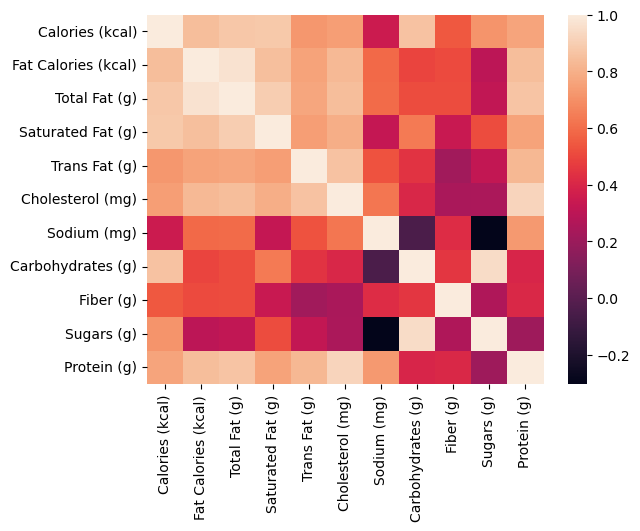
\includegraphics[width=0.75\textwidth]{images/heatmap.png}
        \caption{Тепловая карта корреляции параметров набора данных}
    \end{figure}

    \begin{figure}[H]
        \centering
        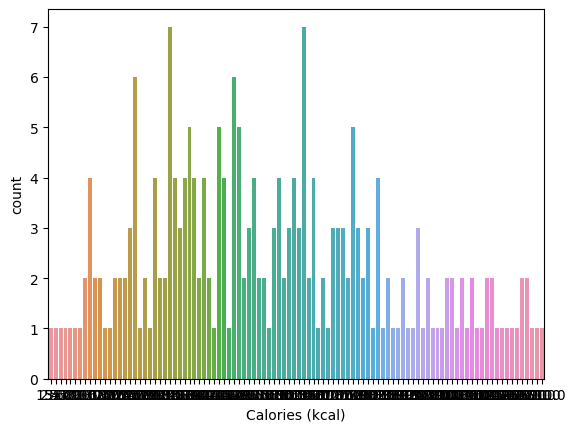
\includegraphics[width=0.75\textwidth]{images/countplot.png}
        \caption{Диаграмма countplot по столбцу <<Calories (kcal)>>}
    \end{figure}

    \section{Заключение}
    
    В рамках задания был успешно загружен датасет. Затем производилось удаление дубликатов и вывод основной информации. Осуществлялись переименование, удаление столбцов, а также их различная визуализация и анализ.

    Данная работа дала начальные навыки обработки и анализа данных с помощью различных, популярных инструментов языка python (pandas, seaborn, scipy).

    \section{Список использованных источников}

    \begin{itemize}
        \item Pandas documentation Date: Nov 22, 2022 Version: 1.5.2
        \item Seaborn. User guide and tutorial
        \item SciPy documentation Date: October 19, 2022 Version: 1.9.3
    \end{itemize}
\end{document}
